\documentclass[a4paper,12pt]{book}
\usepackage[utf8]{inputenc}
\usepackage{pscyr}          % Нормальные шрифты
\usepackage[russian]{babel} %
\usepackage{graphicx}
\usepackage[left=2cm,right=2cm,top=2cm,bottom=2cm,bindingoffset=0cm]{geometry}
\usepackage{wrapfig}   % обтекаемые текстом блоки
\usepackage{soulutf8}  % выделение текста
\usepackage{xcolor}    % выделение цветом
\usepackage{array}
\usepackage{booktabs}
\usepackage{multirow,bigdelim}
\usepackage{hhline}
\usepackage{tabularx}
\usepackage{hyperref}
\usepackage{amsmath,amssymb}
\usepackage{nccboxes}
\usepackage{mathtext}

\hypersetup{pdftitle={Электромагнитные переходные процессы}}  % метаданные PDF
\hypersetup{pdfauthor={Сергей Александрович Ульянов}}
\hypersetup{pdfcreator={LaTeX}}
\hypersetup{pdfproducer={http://ulianov.net}}


%\hypersetup{ pdfborder={0 0 0}} % чтобы ссылки не выделялись

%\usepackage[dvips]{graphicx}
%\graphicspath{{pic/}}

\begin{document}

\author{Сергей Александрович Ульянов}
\title{Электромагнитные переходные процессы}
\date{1970}

\frontmatter
\maketitle
\tableofcontents
\mainmatter

\chapter{Основные сведения об электромагнитных переходных процессах}
\label{chap:1 osnovnye_svedeniia_ob_elektromagnitnykh_perehodnykh_protcessakh}

\section{Основные определения}
\label{sec:1-1 osnovnye_opredeleniia}

Из всего многообразия электромагнитных переходных процессов в электрической системе наиболее распространенными являются процессы, вызванные:
\begin{enumerate} 
	\item
	включением и отключением двигателей и других приемников электроэнергии;
	\item
	коротким замыканием в системе, а также повторным включением и отключением (одновременным или 
каскадным) короткозамкнутой цепи;
	\item
	возникновением местной несимметрии в системе (например, отключение одной фазы линии передачи);
	\item
	несинхронным включением синхронных машин. 
\end{enumerate}

\so{Коротким замыканием} называют всякое не предусмотренное нормальными условиями работы замыкание между фазами, а в системах с заземленными нейтралями (или четырехпроводных)~---  также замыкание одной или нескольких фаз на землю (или на нулевой провод).

В системах с незаземленными нейтралями или с нейтралями, заземленными через специальные компенсирующие устройства, замыкание одной из фаз на землю называют \so{простым замыканием}. При этом виде повреждения прохождение тока обусловлено главным образом емкостью фаз относительно земли.

При возникновении короткого замыкания в электрической системе сопротивление цепи уменьшается (степень уменьшения зависит от положения точки короткого замыкания в системе), что приводит к увеличению токов в отдельных ветвях системы по сравнению с токами нормального режима. в свою очередь это вызывает снижение напряжений в системе, которое особенно велико вблизи места короткого замыкания.

Обычно в месте замыкания образуется некоторое переходное сопротивление, состоящее из сопротивления возникшей электрической дуги и сопротивлений прочих элементов пути тока от одной фазы к другой или от фазы на землю. Электрическая дуга возникает или с самого начала происшедшего повреждения как, например, при перекрытии или пробое изоляции, или через некоторое время, когда перегорит элемент, вызвавший замыкание. При замыканиях между фазами переходное сопротивление определяется главным образом сопротивлением электрической дуги.

\begin{wrapfigure}[17]{r}{0.4\linewidth} % 1-1
	\centering
	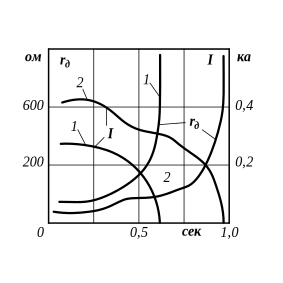
\includegraphics[width=0.95\linewidth]{pic/1-1}
	\caption{Кривые изменения во времени тока и сопротивления самопогасающей открытой дуги на линии 110~\textit{кв} с деревянными опорами. \textit{1, 2} -- номера опытов.}
	\label{fig:1-1 r_i_I}
\end{wrapfigure}


Когда токи достаточно велики (сотни ампер и более), сопротивление дуги приблизительно постоянно и по своему характеру почти чисто активное. С уменьшением, тока и увеличением длины дуги, что имеет место в течение переходного процесса, ее сопротивление возрастает. Наглядной иллюстрацией такого изменения могут служить графики (рис.~\ref{fig:1-1 r_i_I}), полученные экспериментально при возникновении самопогасающих дуг на линиях 110~\textit{кв} с деревянными опорами.

В ряде случаев переходные сопротивления могут быть столь малы, что практически ими можно пренебречь. Такие замыкания называют \so{металлическими}.

Естественно, при прочих равных условиях ток при металлическом замыкании больше, чем при наличии переходного сопротивления. Поэтому, когда требуется найти возможные наибольшие величины токов, исходят из наиболее тяжелых условий, считая, что в месте замыкания отсутствуют какие-либо переходные сопротивления\footnote{Учет переходных сопротивлений и контактных соединений при выполнении расчетов коротких замыканий для установок напряжением до 1000~\textit{в} имеет особое значение (\colorbox{red}{§~17-5}).}.

В трехфазных системах с заземленной нейтралью различают следующие основные виды коротких замыканий в одной точке:

\begin{enumerate} 
	\item
	трехфазное;
	\item
	двухфазное;
	\item
	однофазное;
	\item
	двухфазное на землю, т.~е, замыкание между двумя фазами с одновременным замыканием той же точки на землю. 
\end{enumerate}

Трехфазное короткое замыкание является симметричным, так как при нем все фазы остаются в одинаковых условиях\footnote{При наличии переходных сопротивлений симметрия сохраняется лишь при равенстве этих сопротивлений.} Напротив, все остальные виды коротких замыканий являются несимметричными, поскольку при каждом из них фазы находятся уже в неодинаковых условиях; поэтому системы токов и напряжений при этих видах короткого замыкания в той или иной мере искажены.
	
Многолетняя аварийная статистика по союзным и зарубежным системам показывает, что при глухозаземленной нейтрали относительная вероятность различных основных видов короткого замыкания характеризуется примерными данными табл. \ref{tabl:1-1 veroiatnost_kz} В той же таблице показаны рекомендуемые сокращенные обозначения каждого вида короткого замыкания.

Как видно из этой таблицы, подавляющее число коротких замыканий связано с замыканием на землю, в то время как трехфазное короткое замыкание является очень редким. Однако отсюда было бы неправильным делать вывод, что трехфазное короткое замыкание можно вообще оставить без внимания. Поскольку оно все же возможно, с ним следует считаться, тем более что оно иногда может быть решающим для окончательного суждения относительно возможности работы в условиях короткого замыкания. Само изучение процесса трехфазного короткого замыкания особенно важно в связи с тем, что применение метода симметричных составляющих позволяет величины токов и напряжений прямой последовательности любого несимметричного замыкания определять как соответственные величины при некоторых условных трехфазных замыканиях.

\begin{table}[h] % 1-1
	\centering
	\begin{tabular}{|>{\centering\arraybackslash}m{0.2\linewidth}|>{\centering\arraybackslash}m{0.32\linewidth}|>{\centering\arraybackslash}m{0.19\linewidth}|>{\centering\arraybackslash}m{0.19\linewidth}|}
		\hline
		Виды короткого замыкания & Принципиальная схема & Буквенное обозначение на схемах места и вида короткого замыкания & Относительная вероятность короткого замыкания, \% \\
		\hline
		Трехфазное & 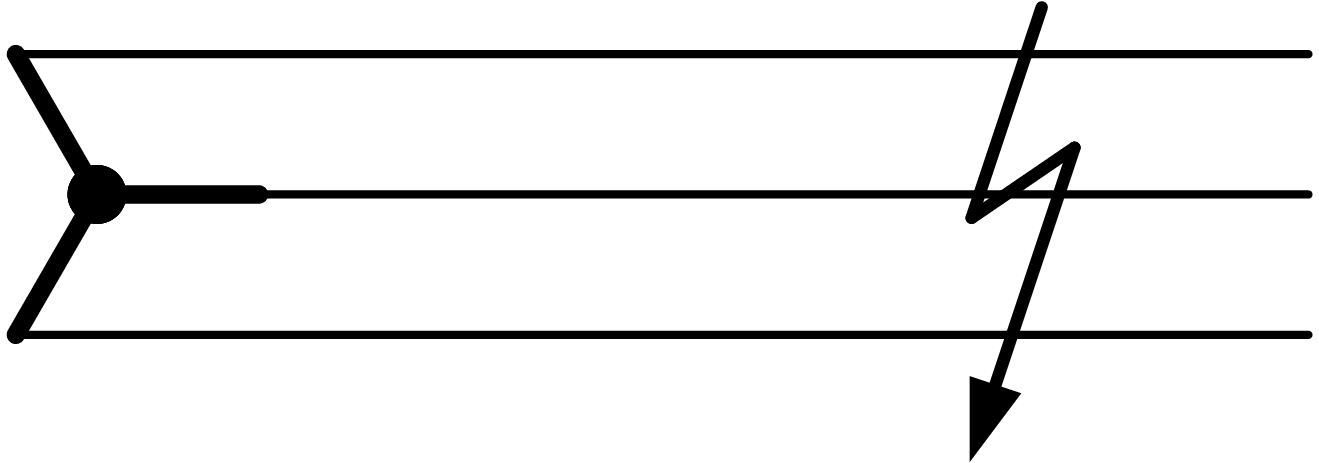
\includegraphics[width=0.7\linewidth]{pic/1-x-1} & $ K^{(3)} $ & 5 \\
		Двухфазное & 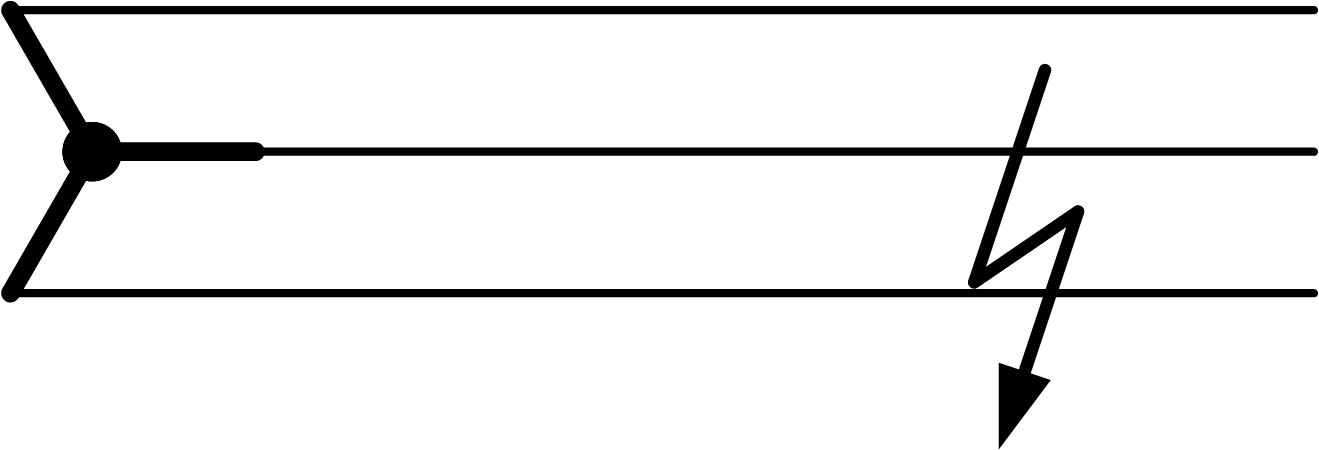
\includegraphics[width=0.7\linewidth]{pic/1-x-2} & $ K^{(2)} $ & 10 \\
		Однофазное & 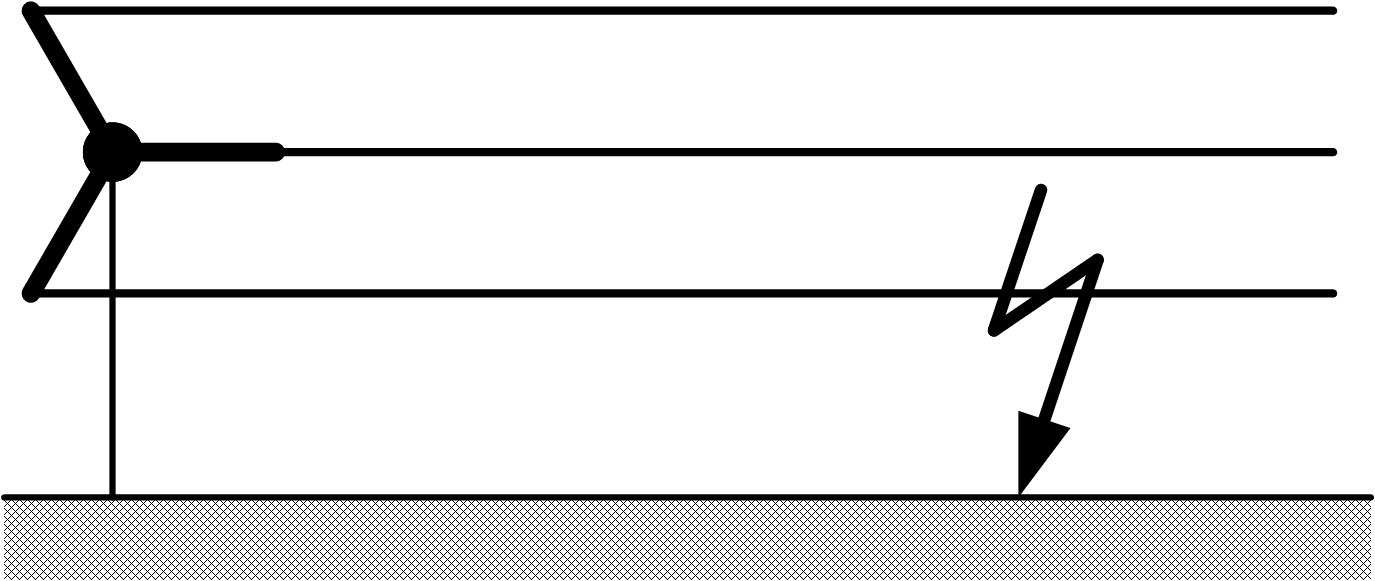
\includegraphics[width=0.7\linewidth]{pic/1-x-3} & $ K^{(1)} $ & 65 \\
		Двухфазное на землю & 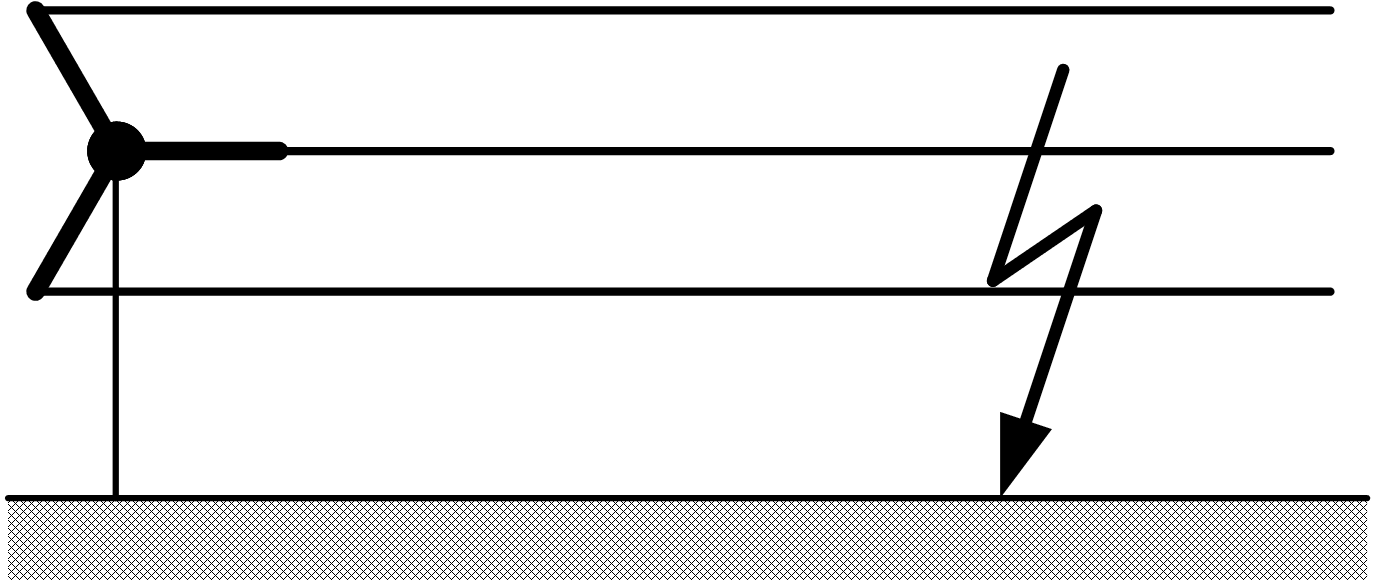
\includegraphics[width=0.7\linewidth]{pic/1-x-4} & $ K^{(1,1)} $ & 20 \\
		\hline
	\end{tabular}
	\caption{Относительная вероятность и сокращенные обозначения основных видов короткого замыкания}
	\label{tabl:1-1 veroiatnost_kz}
\end{table}

Здесь нелишне также отметить, что процесс включения любого трехфазного приемника или невозбужденного синхронного генератора или двигателя можно рассматривать как трехфазное короткое замыкание за некоторым сопротивлением.

Иногда в процессе развития аварии первоначальный вид короткого замыкания переходит в другой вид короткого замыкания. Так, например, в кабельных сетях (с трехжильными кабелями) несимметричные короткие замыкания часто переходят в трехфазные короткие замыкания, так как образовавшаяся при повреждении в кабеле электрическая дуга быстро разрушает изоляцию между его жилами.

Несимметричные короткие замыкания, а также несимметричные нагрузки по существу представляют различные виды \so{поперечной несимметрии}.

Нарушение симметрии какого-либо промежуточного элемента трехфазной цепи (например, отключение одной фазы линии передачи и т.~п.) называют \so{продольной несимметрией}.

Возможны случаи, когда одновременно возникает несколько несимметрий одинакового или различного вида. Так, например, при обрыве провода воздушной линии один его конец, расположенный близко к точке подвеса, остается изолированным, а другой, упав на землю, образует однофазное короткое замыкание. Здесь одновременно возникают продольная и поперечная несимметрии. В качестве другого примера, когда возникают несимметрии одного вида, может служить так называемое \so{двойное замыкание на землю}, т.~е. одновременное замыкание на землю разных фаз в различных точках сети, работающей с изолированной нейтралью.

Все виды повреждений, сопровождающихся мног кратной несимметрией, называют \so{сложными}. К ним, очевидно, относится также любое несимметричное короткое замыкание в сети, работающей в неполнофазном режиме.

Практикой эксплуатации электрических систем установлено, что большая часть возникающих повреждений, особенно на воздушных линиях, имеет проходящий характер, т.~е. повреждения самоустраняются после отключения поврежденного участка и не возникают вновь при обратном включении его. Примером такого самоустраняющегося повреждения может служить обычное перекрытие по поверхности гирлянды изоляторов линии, вызванное грозовым разрядом. После отключения линии электрическая прочность воздушного промежутка восстанавливается в течение небольшого отрезка времени, необходимого для деионизации воздуха в месте перекрытия.

В соответствии с этим широкое применение нашло автоматическое повторное включение (АПВ) цепей и особенно воздушных линий. Поскольку на последних преобладают замыкания одной фазы, у них производят иногда отключение только поврежденной фазы с после дующим однофазным автоматическим повторным включением (ОАПВ). Наконец, помимо однократного выполняют также многократное автоматическое повторное включение с соответствующими интервалами времени его действия.

Наглядной иллюстрацией эффективности автоматического повторного включения служат данные табл.~\ref{tabl:1-1 effekivnost_apv}, представляющие показатели работы устройств автоматического повторного включения по всем союзным энергосистемам за пятилетие 1962--1966~гг. \cite{Zeilndzon69}.

% \cite{Zeilndzon69}  

\begin{table}[h]
	\centering
	\small
	\begin{tabular}{|>{\centering\arraybackslash}p{0.3\textwidth}|>{\centering}p{0.08\textwidth}|>{\centering\arraybackslash}m{0.08\textwidth}|>{\centering\arraybackslash}m{0.08\textwidth}|>{\centering\arraybackslash}m{0.08\textwidth}|>{\centering\arraybackslash}m{0.08\textwidth}|>{\centering\arraybackslash}m{0.08\textwidth}|}
		\hline
		\multirow{3}{*}{\addbox{4ex}{0ex}{Место установки АПВ}} & \multicolumn{4}{c|}{Трехфазное АПВ} & \multicolumn{2}{>{\centering}p{0.2\textwidth}|}{\multirow{2}{*}{ \parbox[c]{0.2\textwidth}{\centering Однофазное АПВ однократного действия}}} \\
		\cline{2-5}
		& \multicolumn{2}{>{\centering}p{0.2\textwidth}|}{однократного действия} & \multicolumn{2}{>{\centering}p{0.2\textwidth}|}{многократного действия} & \multicolumn{2}{c|}{} \\
		\cline{2-7}
		& успешно & неуспешно & успешно & неуспешно & успешно & неуспешно \\
		\hline
		Воздушные линии 1--10~\textit{кв} & 53,5 & 46,5 & 56,2 & 43,8 & --- & --- \\
		То же 20--35~\textit{кв} & 69,5 & 30,5 & 78,1 & 21,9 & --- & --- \\
		110--154~\textit{кв} & 75,0 & 25,0 & 80,5 & 19,5 & 73,2 & 26,8 \\		 
		220--330~\textit{кв} & 76,5 & 23,5 & 77,2 & 22,8 & 80,7 & 19,3 \\
		400-500~\textit{кв} & 67,0 & 33,0 & --- & --- & 59,5 & 40,5 \\
		Смешанные линии & 56,2 & 43,8 & 68,3 & 31,7 & --- & --- \\
		Кабельные линии всех напряжений & 45,3 & 54,7 & 43,0 & 57,0 & --- & --- \\		 		 
		Шины & 64,8 & 25,2 & --- & --- & --- & --- \\		 
		Трансформаторы & 60,0 & 40,0 & --- & --- & --- & --- \\
		\hline
		Средние по всем АПВ данного исполнения & 58,2 & 41,8 & 69,2 & 30,8 & 73,0 & 27,0 \\
		\hline 
	\end{tabular}
	\normalsize
	\caption{Показатели работы автоматического повторного включения по всем энергосистемам Союза за 1962--1966~гг. (в процентах)}
	\label{tabl:1-1 effekivnost_apv}
\end{table}

Как видно, на воздушных линиях относительное число самоустраняющихся повреждений, которому соответствует успешная работа автоматического повторного включения, составляет значительное большинство (преимущественно у линий 20—330~\textit{кв}) всех повреждений на них, причем успешная работа АПВ многократного действия несколько выше, чем однократного действия. Последнее указывает на то, что для самоустранения повреждения иногда требуется больше времени, чем интервал до первого повторного включения.

В кабельных линиях, как и следовало ожидать, число самоустраняющихся повреждений заметно меньше, чем в воздушных. Оно составляет примерно половину общего числа повреждений в кабелях.

Интересно отметить, что даже у трансформаторов больше половины всех повреждений являются самоустраняющимися.

При неуспешном автоматическом повторном включении, т.~е. когда возникшее повреждение в цепи сохранилось, переходный процесс состоит из нескольких этапов. Первый из них наступает в момент возникновения короткого замыкания и продолжается до отключения поврежденного участка. Вторым этапом является пауза (порядка 0,5~\textit{сек} и более) до момента повторного включения, с которого наступает третий этап, продолжающийся до нового отключения того же участка. При многократном автоматическом повторном включении число этапов соответственно возрастает\footnote{Пауза перед вторым повторным включением значительно больше, чем перед первым таким включением. Она определяется характеристиками самого выключателя.}. При применении однофазного автоматического повторного включения в течение паузы перед повторным включением в системе сохраняется местная продольная несимметрия (отключена одна фаза).

Когда повреждение происходит в узле, связывающем несколько цепей, или на участке с двусторонним питанием, переходный процесс дополнительно усложняется тем, что отключение этих цепей или соответственно участка с его обоих концов обычно происходит неодновременно (каскадное отключение).

Каждый из указанных этапов наступает, когда переходный процесс предшествующего этапа еще не закончен. Иными словами, процесс короткого замыкания при неуспешном автоматическом повторном включении состоит из неоднократно сменяющихся переходных процессов.

\so{Форсировка возбуждения} синхронных машин, которую обеспечивают специальные устройства \so{автоматического регулирования возбуждения} (АРВ), происходит при снижении напряжения; обычно оно вызвано каким-либо нарушением нормального режима машины. Следовательно, здесь также на возникший переходный процесс накладывается дополнительный переходный процесс нарастания возбуждения машины.

При повреждении обмоток синхронной машины помимо отключения последней от сети производят быстрое ее развозбуждение путем \so{гашения магнитного поля}. Процесс такого гашения имеет свои особенности и, чтобы обеспечить сохранность машины, на него накладывают определенные ограничения.

\begin{figure}
	\begin{minipage}[h]{1\linewidth}
		\center{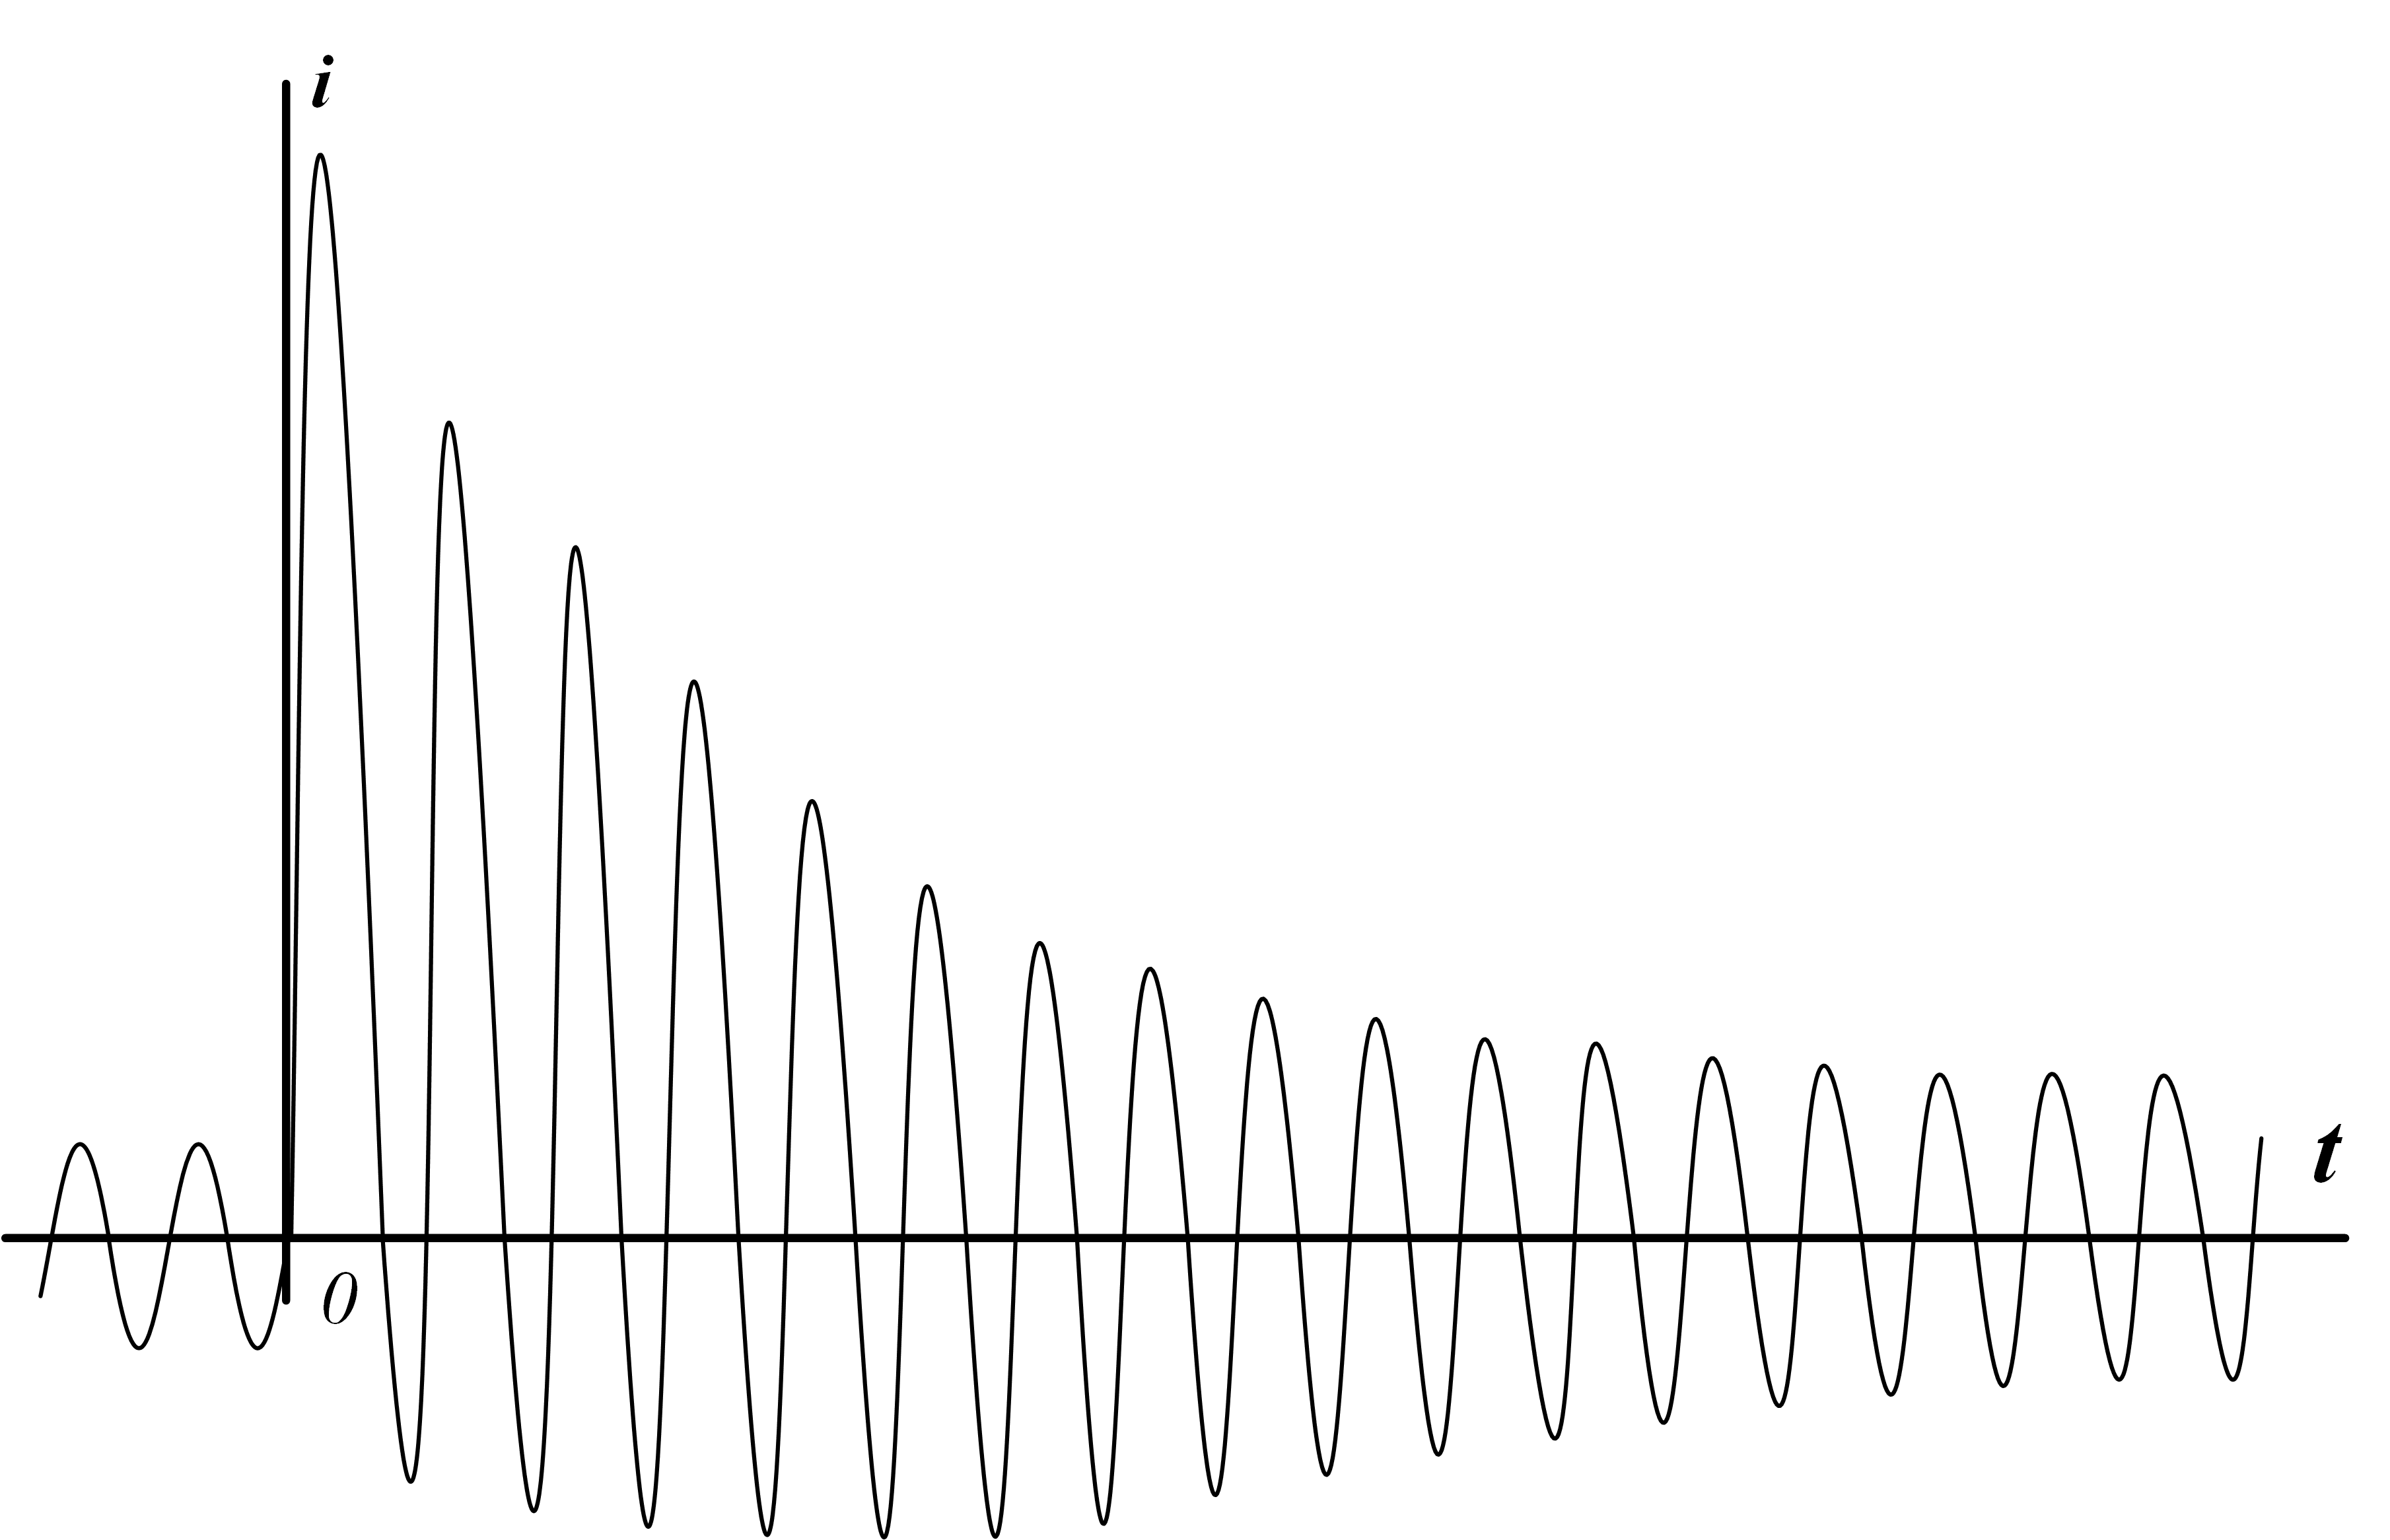
\includegraphics[width=0.7\linewidth]{pic/1-2_a} \\ \textit{а)}}
	\end{minipage}
	\vfill
	\begin{minipage}[h]{1\linewidth}
		\center{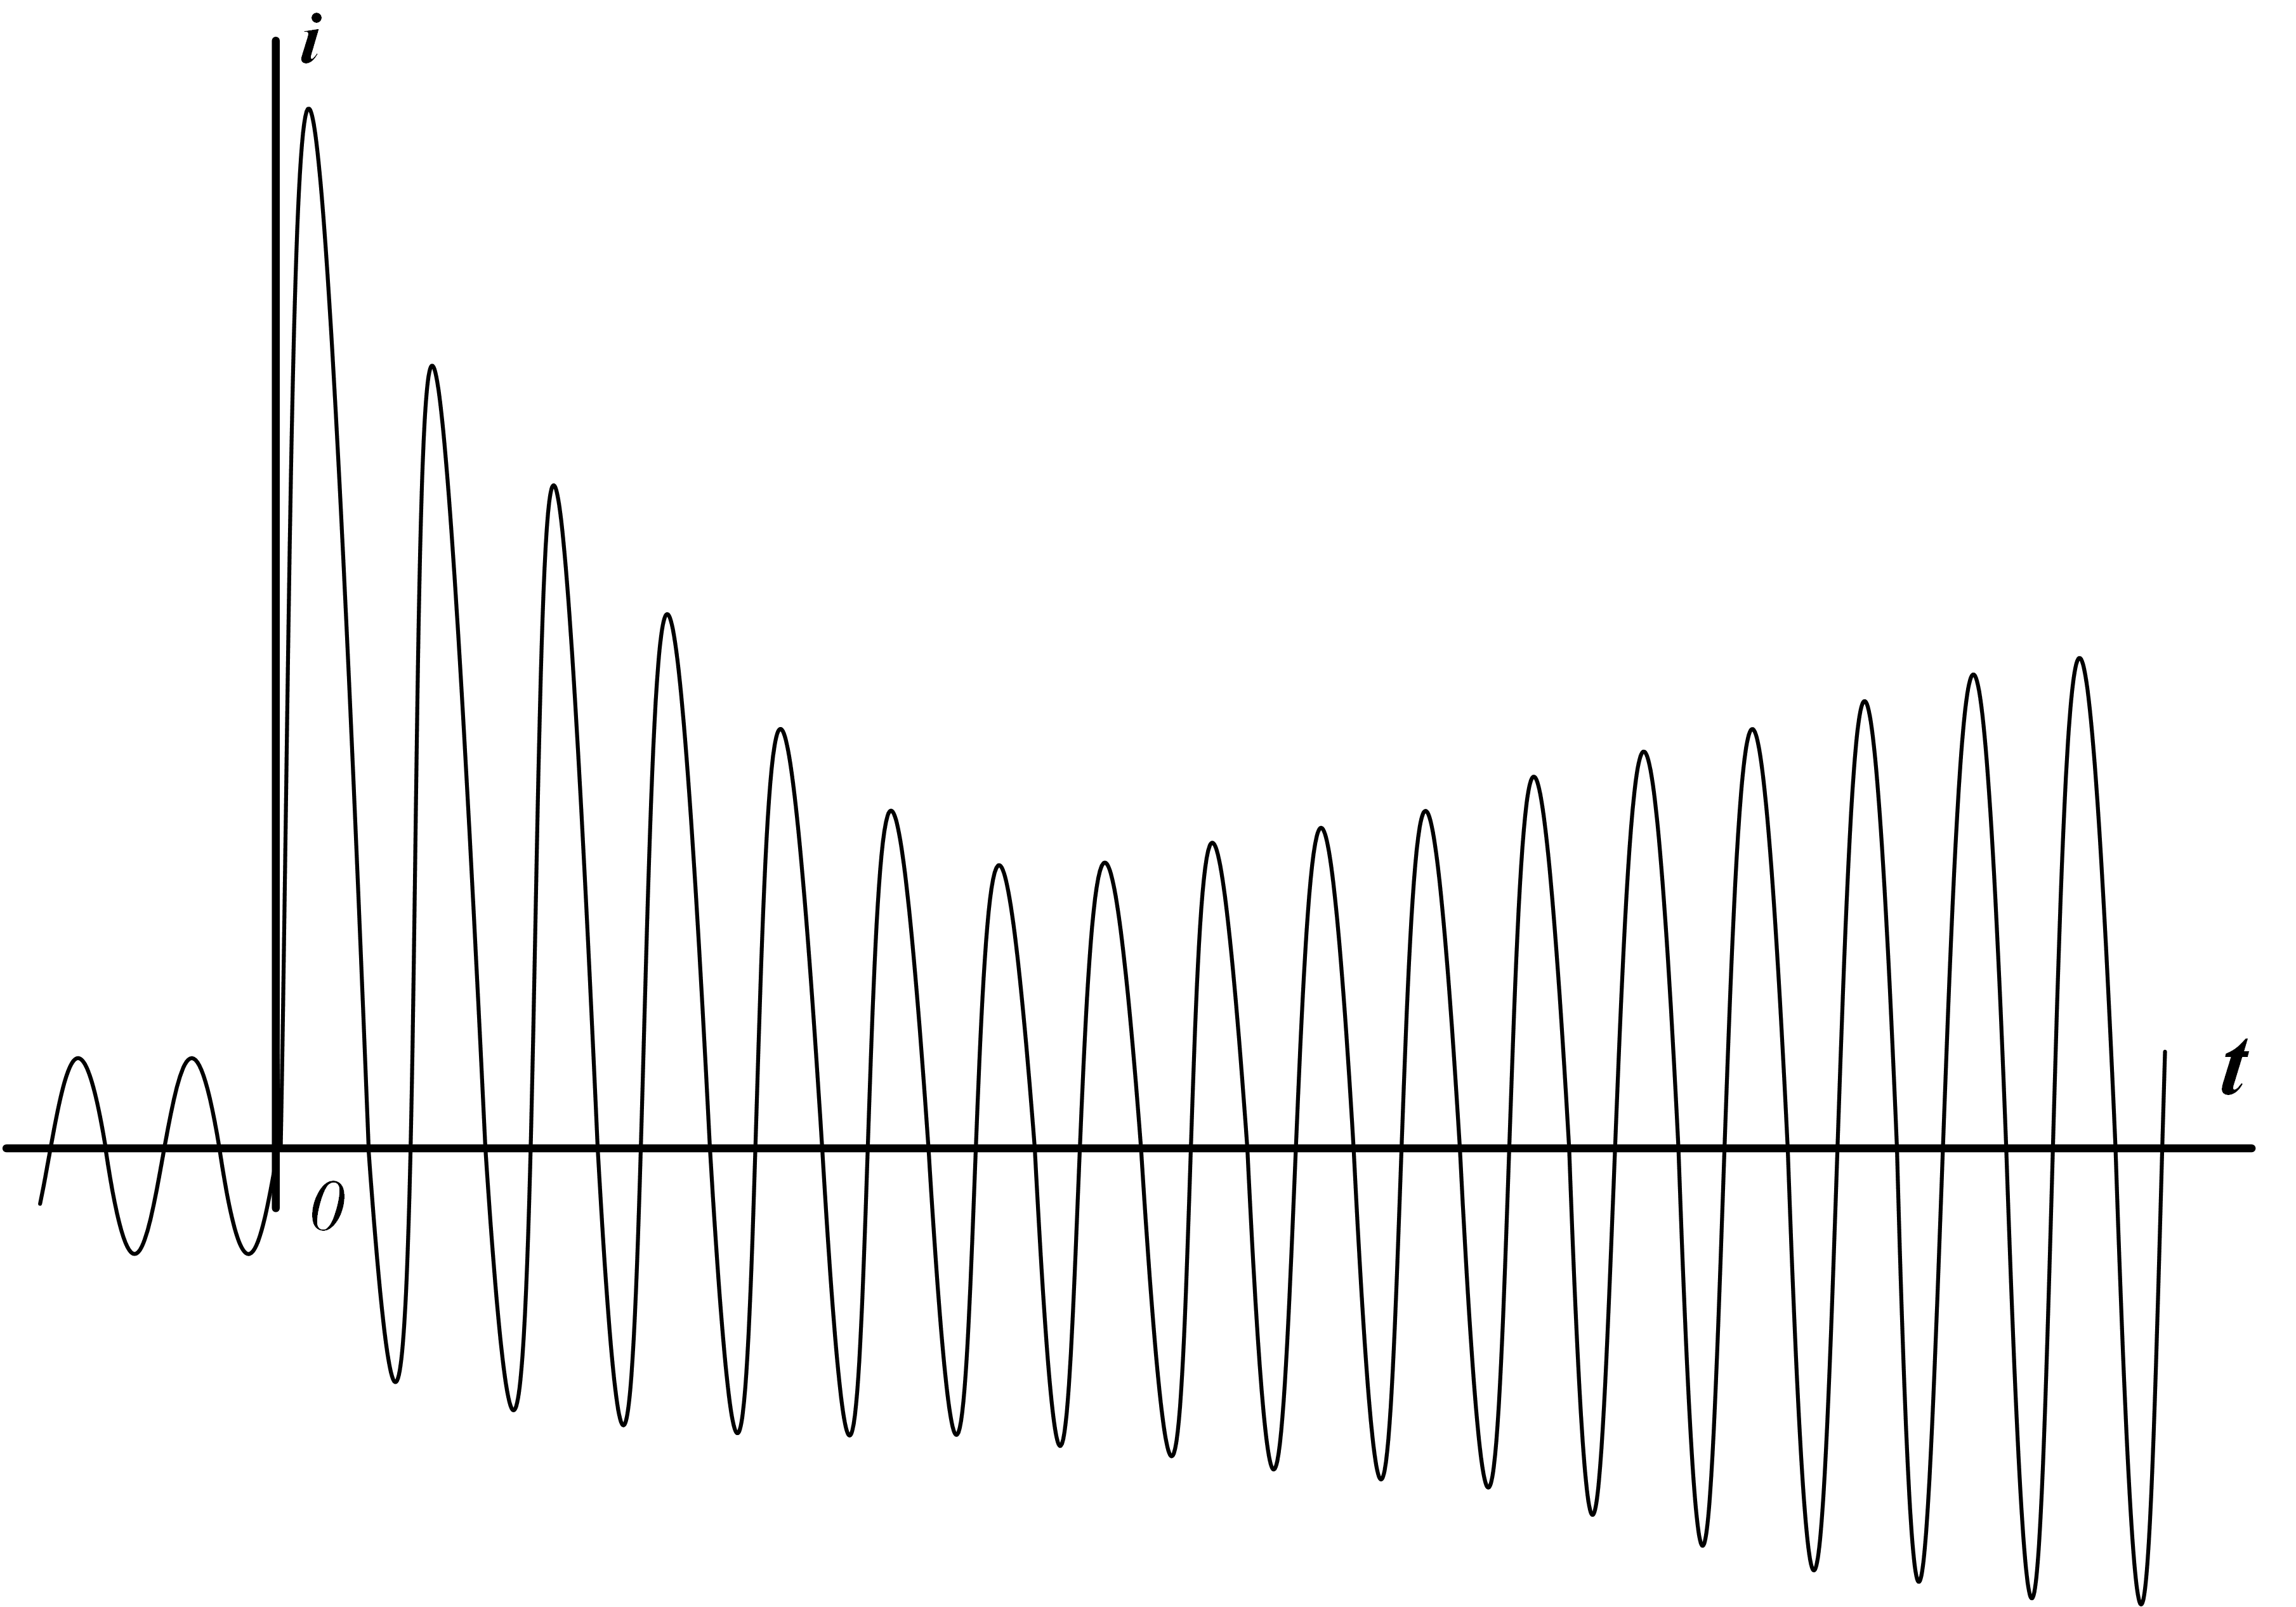
\includegraphics[width=0.7\linewidth]{pic/1-2_b} \\ \textit{б)}}
	\end{minipage}
	\caption{Осциллограммы токов при внезапном коротком замыкании. \textit{а} --- при отстутствии автоматического регулирования возбуждения; \textit{б} --- при наличии такого регулирования.}
	\label{ris:1-2 toki_kz_bez_arv_i_s_nim}
\end{figure}

Для иллюстрации процесса короткого замыкания на рис.~\ref{ris:1-2 toki_kz_bez_arv_i_s_nim} приведены типичные осциллограммы тока короткого замыкания при отсутствии автоматического регулирования возбуждения (рис.~\ref{ris:1-2 toki_kz_bez_arv_i_s_nim},а) и при наличии его (рис.~\ref{ris:1-2 toki_kz_bez_arv_i_s_nim},б). В начальной стадии обе осциллограммы практически одинаковы. Это объясняется тем, что здесь их характер определяется главным образом затуханием возникших свободных токов, а нарастание тока возбуждения от действия АРВ благодаря магнитной инерции еще очень мало. В дальнейшем, как видно, при отсутствии АРВ кривая постепенно переходит в синусоиду нового установившегося режима. При наличии АРВ амплитуда кривой тока, достигнув некоторого наименьшего значения, вновь возрастает, стремясь к установившемуся значению, которое, естественно, больше, чем при отсутствии АРВ. Возрастающий характер кривой тока при наличии АРВ обычно получается при заметной удаленности короткого замыкания относительно генератора.

Для дополнительной иллюстрации характерных переходных процессов приведем еще несколько осциллограмм. На рис. 1-3 показаны осциллограммы токов в фазе статора, обмотке возбуждения и продольной демпферной обмотке синхронного генератора мощностью 50~\textit{Мвт} при внезапном трехфазном коротком замыкании на его выводах. До короткого замыкания генератор работал на холостом ходу и его АРВ было отключено. На \colorbox{red}{рис. 1-4} приведены осциллограммы тока фазы статора асинхронного двигателя 600~\textit{квт} и потребляемой им активной мощности при трехфазном коротком замыкании вблизи двигателя и при его дальнейшем самозапуске после отключения короткого замыкания (спустя примерно 1,2~\textit{сек}).

\section{Причины возникновения и следствия}
\label{sec:1-2 prichiny_vozniknoveniia_i_sledstviia}

Основной причиной возникновения рассматриваемых в дальнейшем электромагнитных переходных процессов являются преимущественно короткие замыкания. Последние в свою очередь являются результатом нарушений изоляции электрического оборудования, которые вызываются старением изоляционных материалов, перенапряжениями, недостаточно тщательным уходом за оборудованием и непосредственными механическими повреждениями (например, повреждение кабеля при выполнении земляных работ без должной осторожности и т.~п.). В практике наблюдались случаи, когда короткие замыкания возникали от перекрытия токоведущих частей животными и птицами.

При осуществлении упрощенных схем электрических соединений понижающих подстанций, как известно, используют специальные аппараты --- короткозамыкатели (одно- и двухфазные); последние создают преднамеренные короткие замыкания с целью быстрых отключении ранее возникших повреждений.

Таким образом, наряду с короткими замыканиями случайного характера в системе имеют место также преднамеренные короткие замыкания, вызываемые действием установленных короткозамыкателей.

Социалистическое хозяйство предъявлёт особые требования к безаварийному электроснабжению всех потребителей электроэнергии. Поэтому внимание и усилия работников в области электроэнергетики должны быть направлены на соблюдение этих требований. Для этого должно быть в первую очередь обеспечено строгое соблюдение Правил технической эксплуатации электрических установок. Помимо того, требуется непрерывное повышение качества продукции, выпускаемой электротехнической промышленностью.

В зависимости от места возникновения и продолжительности повреждения его последствия могут иметь местный характер или, напротив, могут отражаться на всей системе.

Так, например, при коротком замыкании в удаленной точке сети величина тока короткого замыкания составляет лишь незначительную долю номинального тока питающих генераторов и возникновение такого короткого замыкания воспринимается ими как небольшое увеличение нагрузки. Сильное снижение напряжения получается вблизи места трехфазного короткого замыкания, в то время как в других точках системы наблюдается едва заметное снижение напряжения, причем от действия автоматического регулирования возбуждения оно быстро восстанавливается до нормального. Следовательно, при рассматриваемых условиях опасные последствия короткого замыкания проявляются лишь в ближайших к месту короткого замыкания частях системы.

Аналогичная картина, но выраженная не в столь резкой форме, наблюдается при пуске крупных двигателей, синхронных компенсаторов, при включении генераторов способом самосинхронизации, а также при их несинхронном включении.

Обрыв фазы слабо загруженной цепи, очевидно, не вызовет каких-либо существенных изменений режима в системе. Напротив, такой обрыв в цепи с большим нагрузочным током может привести к весьма существенным изменениям токов и напряжений в системе.

Ток короткого замыкания даже в тех случаях, когда он мал по сравнению с номинальным током генератора, обычно во много раз превышает номинальный ток самой самой ветви, поэтому и при кратковременном прохождении тока короткого замыкания он может вызвать дополнительный нагрев токоведущих элементов и проводников выше допустимого.

Кроме теплового действия, токи короткого замыкания вызывают между проводниками большие механические усилия, которые особенно велики в начальной стадии процесса короткого замыкания, когда ток достигает максимума. При недостаточной прочности проводников и их креплений они могут быть разрушены при коротком замыкании. Равным образом это относится к электрическим машинам и аппаратам, надежность которых может быть обеспечена при учете всех проявлений коротких замыканий.

Глубокое снижение напряжения и резкое искажение его симметрии, которое возникают при коротких замыканиях и образовании продольной несимметрии, вредно отражаются иа работе потребителей. Так, уже при понижении напряжения на 30--40\% в течение 1~\textit{сек} и более достаточно загруженные двигатели промышленного предприятия могут остановиться, что вызовет народнохозяйственный ущерб. Оставаясь включенными в сеть, остановившиеся двигатели могут вызвать дальнейшее снижение напряжения в сети, т.~е. полное нарушение нормального электроснабжения не только данного предприятия, но и за его пределами. Следует подчеркнуть, что ряд промышленных производств вообще не допускает никаких (даже кратковременных) перерывов в подаче энергии.

При замыканиях на землю возникают неуравновешенные системы токов. Они способны создавать магнитные потоки, которые достаточны, чтобы в соседних линиях связи и сигнализации навести э.~д.~с, величины которых могут быть опасны для обслуживающего персонала и аппаратуры этих линий. Заметные мешающие влияния на линии связи возникают также при продольной несимметрии в системе.

Наконец, при задержке отключения короткого замыкания сверх допустимой продолжительности может произойти нарушение устойчивости электрической системы, что является в сущности одним из наиболее опасных последствий короткого замыкания, так как отражается на работе всей системы.

\section{Назначения расчетов и требования к ним}
\label{sec:1-3 naznacheniia_raschetov_i_trebovaniia_k_nim}

При проектировании и эксплуатации электрических установок и систем для решения многих технических вопросов и задач задач требуется предварительно произвести ряд расчетов, среди которых заметное место занимают расчеты электромагнитных переходных процессов и, в частности, процессов при внезапном коротком замыкании.

Под расчетом электромагнитного переходного процесса обычно понимают вычисление токов и напряжений в рассматриваемой схеме при заданных условиях. В зависимости от назначения такого расчета находят указанные величины для заданного момента времени или находят их изменения в течение всего переходного процесса. При этом решение обычно проводится для одной или нескольких ветвей и точек схемы.

К числу задач, для практического решения которых производят такие расчеты, относятся:

\begin{enumerate} 
	\item
	сопоставление, оценка и выбор схемы электрических соединений как отдельных установок (станций, подстанций), так и системы в целом;
	\item
	выявление условий работы потребителей при аварийных режимах;
	\item
	выбор аппаратов и проводников и их проверка по условиям работы при коротких замыканиях;
	\item
	проектирование и настройка устройств релейной защиты и автоматизации;
	\item
	определение условий несинхронного включения синхронных машин и включения их способом самосинхронизации;
	\item
	конструктивные решения элементов распределительных устройств и, в частности, шинопроводов на большие рабочие токи;
	\item
	определение числа заземленных нейтралей и их размещения в системе;
	\item
	выбор числа и мощности компенсирующих дугогасящих устройств;
	\item
	определение влияния линий электропередачи на провода связи и сигнализации;
	\item
	проектирование и проверка защитных заземлений;
	\item
	подбор характеристик разрядников для защиты от перенапряжений (включая защиту конденсаторов установок продольной компенсации);
	\item
	оценка и определение параметров гашения поля синхронных машин;
	\item
	оценка и выбор систем возбуждения синхронных машин;
	\item
	проведение различных испытаний;
	\item
	анализ происшедших аварий.
\end{enumerate}

Особенностью расчетов при решении задач, встречающихся в эксплуатации, является необходимость учета конкретных условий рассматриваемого переходного процесса. Напротив, при проектировании часто довольствуются приближенными данными. Поэтому в первом случае требуется большая точность.

Так, например, благодаря тому, что интервалы между параметрами, характеризующими различные типы аппаратов в отношении их устойчивости при коротких замыканиях, достаточно большие, точность расчета для выбора таких аппаратов может быть невелика. Напротив, точность расчета для целей релейной защиты и автоматизации обычно должна быть значительно выше. Здесь, как впрочем и я ряде других случаев, часто требуется выявлять как наибольшие, так и наименьшие возможные величины токов и напряжений, сдвиг между ними в отдельных фазах или между отдельными их симметричными составляющими, их распределение в схеме и т.~п.

Неменьшие требования предъявляются к расчетам для анализа аварий, а также к расчетам, проводимым для различных исследовательских целей.

Краткие сведения о расчетных условиях даны в~§\ref{sec:2-2 poniatie o raschetnykh usloviiakh}.



















\chapter{Общие указания к выполнению расчетов}

\section{Основные допущения}

Как отмечалось выше, расчет электромагнитного переходного процесса в современной электрической системе с учетом всех имеющих место условий и факторов чрезвычайно сложен и практически невыполним. Поэтому, чтобы упростить задачу и сделать ее решение практически возможным, вводят ряд допущений. Последние зависят прежде всего от характера и постановки самой задачи. Те допущения, которые вполне пригодны при решении одной задачи, могут быть совершенно неприемлемыми при решении другой.

Каждый из практических методов расчета, электромагнитных переходных процессов, в частности процесса при коротком замыкании, основан на некоторых допущениях, касающихся преимущественно возможности использование упрощённых представлений об изменении свободных токов в сложных схемах с несколькими источниками, о разных способах учета автоматического регулирования возбуждения синхронных машин и т.~п. C ними читатель познакомится в ходе дальнейшего изложения материала. Здесь же остановимся только на тех основных допущениях, которые обычно принимают при решении большинства практических задач, связанных с определением токов и напряжений при электромагнитных переходных процессах. К  числу таких допущений следует отнести:

\begin{enumerate} 
	\item
	отсутствие насыщения магнитных систем. При этом все схемы оказываются линейными, расчет которых значительно проще; в частности, здесь могут быть использованны любые формы принципа наложения.
	\item
	Пренебрежение токами намагничивания трансформаторов и автотрансформаторов. Единственным исключением их этого допущения является случай, когда трехстержневой трансформатор с соединением обмоток $ Y_{0}/Y_{0} $ включен на напряжение нулевой последовательности (см.~\colorbox{red}{§12-5}).
	\item
	Сохранение симметрии трехфазное системы. Оня нарушается обычно лишь для какого-либо одного элемента, что происходит в результату его повреждения, или преднамеренно по специальным соображениям (см. гл.~\colorbox{red}{15}).
	\item
	Пренебрежение емкостными проводимостями. Это допущение обычно является, уместным и заметно не искажает результаты решения, если в рассматриваемой схеме нет продольной компенсации индуктивности цепи, а также дальних линий передач напряжением выше 220~\textit{кв}. При рассмотрении простых замыканий на землю (см.~§\colorbox{red}{17-2}) это допущение, разумеется, совсем непригодно, так как в данном случае ток замыкается именно через емкостные проводимости.
	\item
	Приближенный учет нагрузок. В зависимости от стадии переходного процесса нагрузку приближенно характеризуют некоторым постоянным сопротивлением, обычно чисто индуктивным (см.~\colorbox{red}{§5-4 и §6-5}).
	\item
	Отсутствие активных сопротивлений. Это допущение в известной мере условно. Оно приемлемо при определении начальных и конечных значений отдельных величин, характеризующих переходный процесс в основных звеньях высокого напряжения электрической системы; при этом приближенный учет активных сопротивлений находит отражение при оценке постоянных времени затухания свободных составляющих рассматриваемых величин. В тех же случаях, когда подобный расчет проводится для протяженной кабельной или воздушной сети с относительно небольшими сечениями проводников (особенно линии со стальными проводами), а также для для установок и сетей напряжением до 1~\textit{кв}, данное допущение непригодно (см.~\colorbox{red}{гл. 17}).
	\item
	Отсутствие качаний синхронных машин. Если задача ограничена рассмотрением лишь начальной стадии переходного процесса (т.~е. в пределах 0,1--0,2~\textit{сек} с момента нарушения режима до отключения повреждения), это допущение обычно не вносит заметной погрешности (особенно в токе в месте повреждения). Однако при возникновении существенных качаний или выпадении машин из синхронизма достаточно надежный результат может быть получен лишь с учетом (хотя бы приближенным) такого процесса (см.~\colorbox{red}{гл. 19}).
\end{enumerate}

\section{Понятие о расчетных условиях}

В соответствии с целевым назначением проводимого на практике расчета электромагнитного переходного процесса устанавливают исходные расчетные условия. Они весьма разнообразны и при решении разных задач могут быть даже противоположными.

Так, например, для выбора выключателя по условиям его работы при коротком замыкании должны быть определены соответствующие возможные наибольшие величины тока короткого замыкания. С этой целью исходят из предположения, что короткое замыкание происходит в то время, когда включено наибольшее число генераторов, что вид короткого замыкания такой, при котором ток достигает наибольшей величины, что короткое замыкание металлическое и что оно произошло непосредственно у выводов самого выключателя. Помимо того, здесь устанавливают расчетное время размыкания контактов выключателя и цикл производимых им операций (включение и отключение).

Для выбора трубчатого разрядника требуется знать не только наибольшую, но и возможную наименьшую величину тока короткого замыкания, для определения которой, разумеется, должны быть приняты совсем иные расчетные условия.

Большое разнообразие расчетных условий встречается при выполнении расчетов для выбора и настройки устройств релейной защиты и автоматики. В них устанавливаются исходные предшествующие режимы заданной системы, число и расположение заземленных нейтралей, виды повреждений, и последовательность отключения поврежденного участка и т.~п.

При решении вопроса гашения поля синхронной машины в качестве расчетного режима может быть как режим короткого замыкания, так и холостого хода.

Приведенные примеры показывают, сколь велико разнообразие расчетных условий. Обоснование расчетных условий для конкретных технических задач (с учетом вероятности отдельных факторов) является одним из важных вопросов соответствующих специальных дисциплин.

\section{Система относительных единиц}

Представление любых физических величин не в обычных для них соответствующих именованных единицах, а в относительных, безразмерных единицах позволяет существенно упростить некоторые теоретические выкладки и придать им более общий характер. Равным образом и в практических расчетах такое представление величин придает результатам большую наглядность и позволяет быстрее ориентироваться в порядке определяемых значений. Благодаря этому система относительных единиц широко используется, хотя на первый взгляд она может казаться несколько искусственной и даже излишней.

С выражением величин в относительных единицах (в долях или процентах) читатель уже встречался при изучении электрических машин, где реактивности обычно выражают в долях единицы, напряжения короткого замыкания трансформаторов --- в процентах, пусковые токи и моменты асинхронных двигателей --- в кратностях от их номинальных значений и т.~д. Теперь нам нужно познакомиться с системой относительных единиц в более широком аспекте, имея в виду использование ее при решении различных вопросов и задач для схем с произвольным числом всевозможных элементов.

Напомним, что под относительным значением какой-либо величины следует понимать ее отношение к другой одноименной величине, выбранной за единицу измерения. Следовательно, чтобы выразить отдельные величины в относительных единицах, нужно прежде всего выбрать те величины, которые должны служить соответственными единицами измерения, или, как говорят, установить базисные единицы (или условия).

Пусть за базисный ток и базисное междуфазное напряжение приняты некоторые произвольные величины $ I_{\mbox{б}} $ и $ U_{\mbox{б}} $. Тогда базисная мощность трехфазной системы, очевидно, будет:

\begin{equation}
	\label{eq:chap2 S_baz}
	S_{\mbox{б}} = \sqrt{3}U_{\mbox{б}}I_{\mbox{б}}
\end{equation}

и базисное сопротивление

\begin{equation}
	\label{eq:chap2 z_baz}
	z_{\mbox{б}} = \frac{U_{\mbox{б}}}{\sqrt{3}I_{\mbox{б}}}
\end{equation}

т.~е. оно подчинено закону Ома, чтобы обеспечить тождественную запись этого закона как в именованных, так и в относительных единицах.

Как видно, из четырех базисных единиц $ I_{\mbox{б}} $, $ U_{\mbox{б}} $, $ S_{\mbox{б}} $ и $ z_{\mbox{б}} $ только две могут быть выбраны произвольно, а две другие уже получаются из указанных соотношений. Фазные и междуфазные базисные напряжения, а также фазные и линейные базисные токи связаны между собой известными соотношениями для симметричной трехфазной системы. Следует особо подчеркнуть, что выбранные базисные единицы служат для, измерения как полных величин, так и их составляющих (активных, реактивных и~пр.).

% 29 страница









%TODO: Раздел второй - ЭЛЕКТРОМАГНИТНЫЕ ПЕРЕХОДНЫЕ ПРОЦЕССЫ ПРИ СОХРАНЕНИИ СИММЕТРИИ ТРЕХФАЗНОЙ ЦЕПИ
\chapter{Переходный процесс в простейших трехфазных цепях}
\label{chap:3 perehodnyi_protcess_v_prosteishikh_trekhfaznykh_tcepiakh}

\section{Постановка задачи и ее ограничения}
\label{sec:3-1 postanovka_zadachi_i_ee_ogranicheniia}

Симметричную трехфазную цепь с сосредоточенными активными сопротивлениями и индуктивностями при отсутствии в ней трансформаторных связей условимся называть \so{простейшей} трехфазной цепью.

Электромагнитный переходный процесс в такой цепи рассмотрим сначала при условии, что ее питание осуществляется от источника, сопротивление которого равно нулю и его напряжение, изменяясь с постоянной частотой, имеет неизменную амплитуду\footnote{Применение чувствительного и быстродействующего автоматического регулировании возбуждения генераторов дополнительно способствует принятию указанного предположения.}. Обычно его называют источником бесконечной  мощности.

Включение в схему такого источника, вообще говоря, соответствует теоретическому пределу, когда изменение внешних условий не влияет на работу самого источнику. Практически это имеет место, например, при коротких замыканиях в относительно маломощных электрических установках или протяженных сетях, питаемых от крупных энергетических систем (см.~\colorbox{red}{гл. 17}).

С исследованием переходных процессов в подобных условиях читатель знаком из курса теоретических основ электротехники. Поэтому задачей данной главы является кратко напомнить основные выводы такого исследования, отметить особенности многофазной цепи по сравнению с однофазной, привести некоторые упрощенные приемы расчета и обратить внимание на влияние ряда факторов.

\section{Трехфазное короткое замыкание в неразветвленной цепи}
\label{sec:3-2 trekhfaznoe_korotkoe_zamykanie_v_nerazvetvlennoi_tcepi}

Обратимся к рис.~\ref{ris:3-1 simple_3_phase_circut}, на котором представлена простейшая симметричная трехфазная цепь. В ней условно принято, что на одном ее участке имеется взаимоиндукция между фазами, а на другом она отсутствует. Цепь присоединена к источнику синусоидального напряжения с неизменными амплитудой и частотой.

Рассмотрим переходный процесс, вызванный включением выключателя \textit{B}, за которым сделана закоротка, что равносильно возникновению металлического трехфазного короткого замыкания между двумя участками данной цепи.

\begin{figure}[h]
	\center{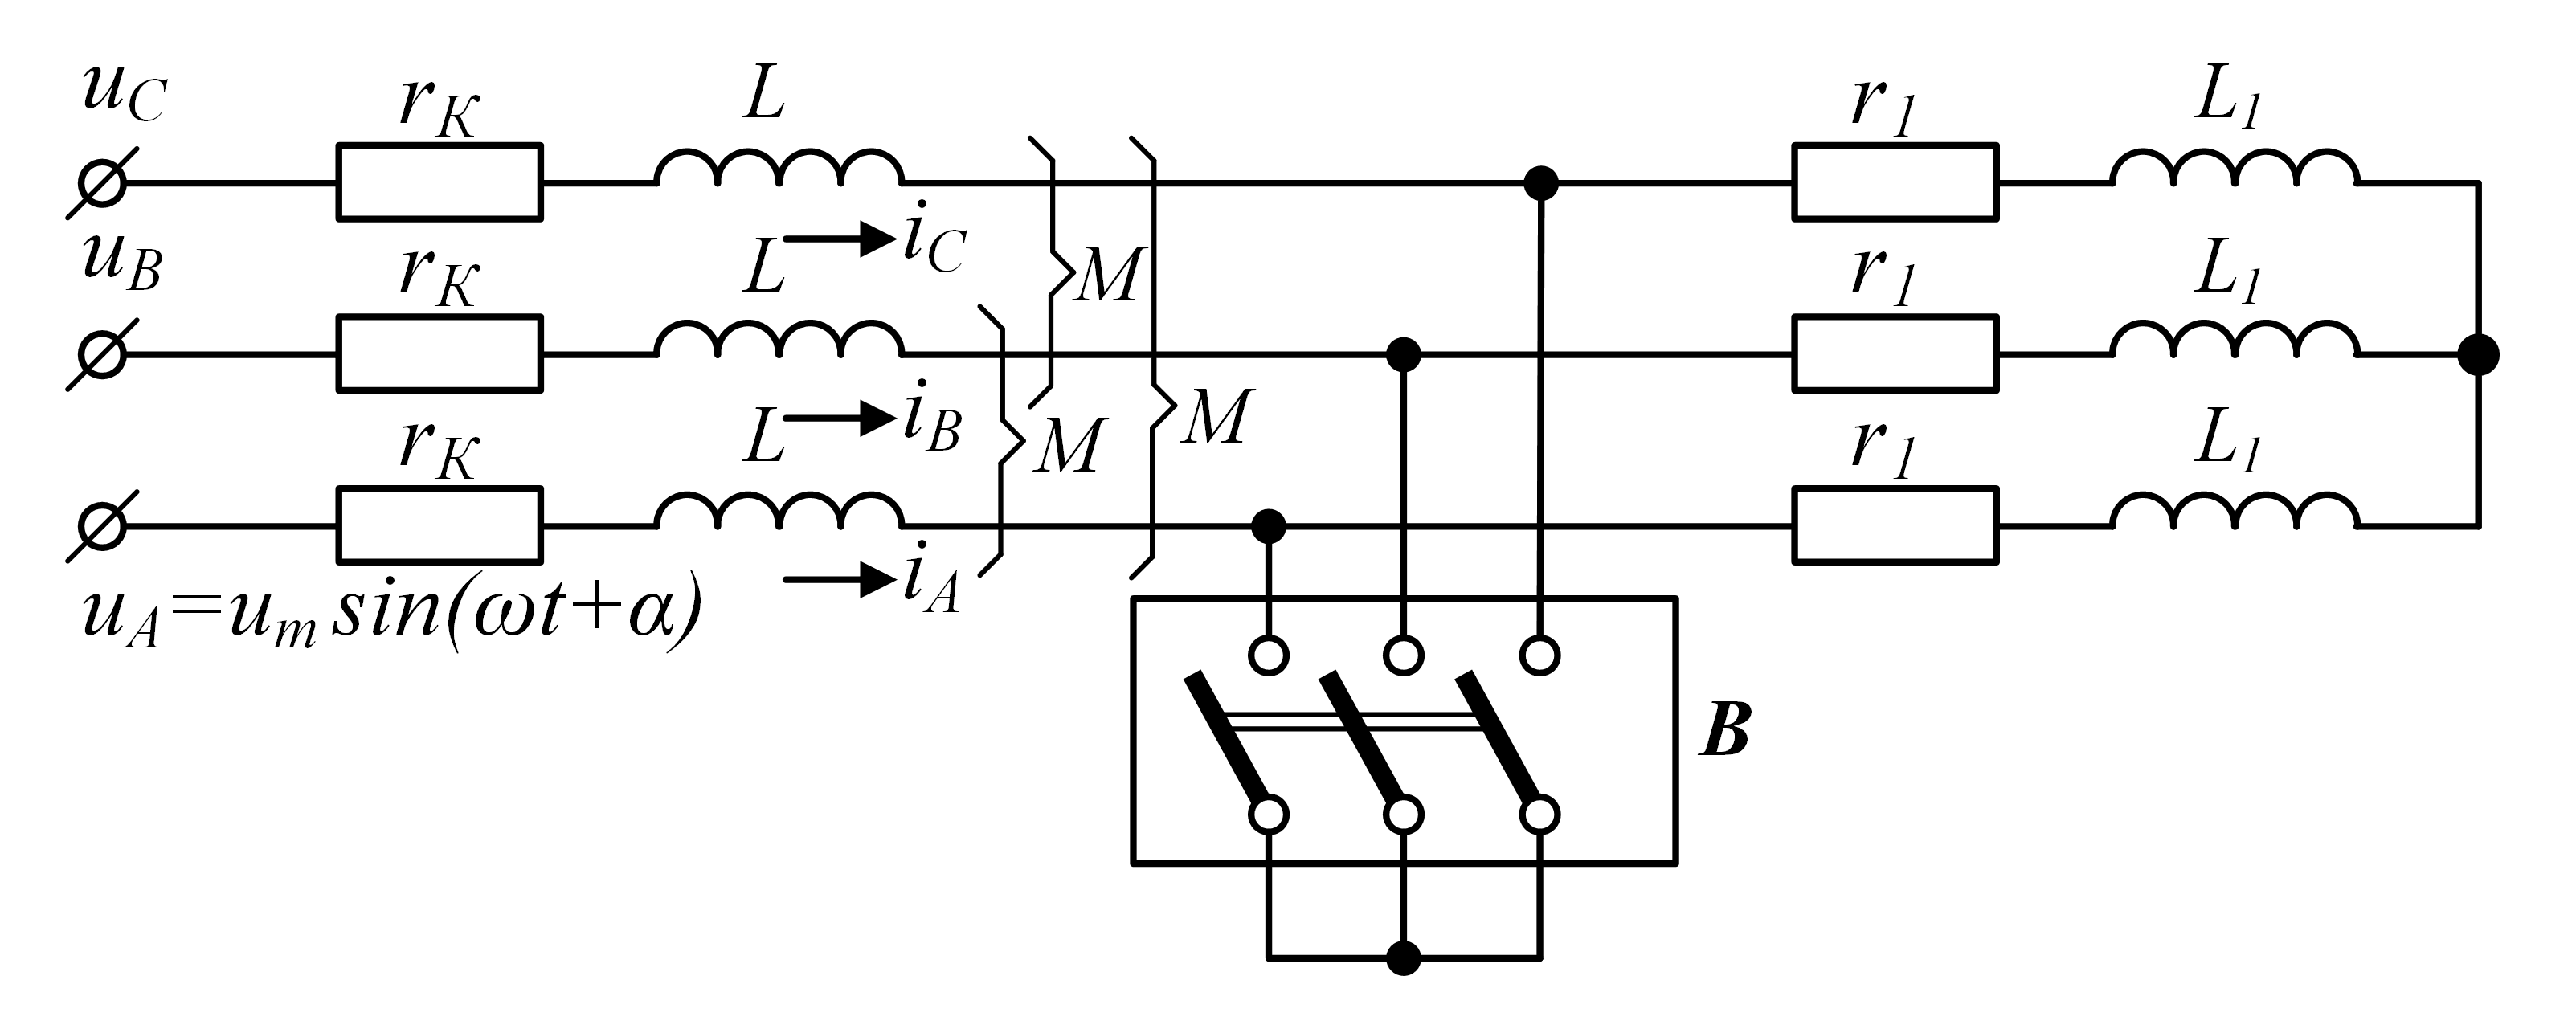
\includegraphics[width=0.9\linewidth]{pic/3-1}}
	\caption{Простейшая трехфазная электрическая цепь.}
	\label{ris:3-1 simple_3_phase_circut}
\end{figure}

Пусть векторы $ \overset{\;.}{U}_A $, $ \overset{\;.}{U}_B $, $ \overset{\;.}{U}_C $, $ \overset{\;.}{I}_A $, $ \overset{\;.}{U}_B $, $ \overset{\;.}{U}_C $ (рис.~\ref{ris:3-2 diagram})
характеризуют предшествующий режим рассматриваемой цепи, а вертикаль \textit{tt} является неподвижной линией времени, т.~е. мгновенные значения отдельных величии определяются проекциями на эту линию соответствующих вращающихся векторов. Момент возникновения короткого замыкания будем фиксировать значением угла $ \alpha $ (т.~е. \so{фазой включения}) между вектором напряжения фазы \textit{A} и горизонталью. (рис.~\ref{ris:3-2 diagram}.

После включения выключателя \textit{В} цепь рис.~\ref{ris:3-1 simple_3_phase_circut} распадается на два независимых друг от друга участка. Участок с $ r_1 $ и $ L_1 $ оказывается зашунтированным коротким замыканием и ток в нем будет поддерживаться лишь до тех пор, пока запасенная в индуктивности $ L_1 $ энергия магнитного потока не перейдет в тепло, поглощаемое активным сопротивлением $ r_1 $.

Дифференциальное уравнение равновесия в каждой фазе этого участка имеет вид:

\begin{equation}
	0 = ir_1 + L_1 \frac{di}{dt}.
	\label{eq:3-1 diff_ur}
\end{equation}

Его решение общеизвестно:

\begin{equation}
	i = i_0 e^{-t / T_{\text{а}1}}; %TODO: Проверить формулу, какая-то черка в степени
	\label{eq:3-2 diff_solve}
\end{equation}

оно показывает, что здесь имеется лишь свободный ток, который затухает по экспоненте с постоянной времени

\begin{equation}
	T_{\text{а}1} = \frac{L_1}{r_1} = \frac{x_1}{\omega r_1}, \textit{~сек}.
	\label{eq:3-3 T_a1}
\end{equation}

Начальное значение свободного тока в каждой фазе зашунтированного участка цепи, очевидно, равно предшествовавшему мгновенному значению тока, поскольку в цепи с индуктивностью не может произойти внезапного (скачком) изменения тока. В общем случае свободные токи в фазах различны, хотя их затухание, разумеется, происходит с одной и той же постоянной времени. В одной из фаз свободный ток может вообще отсутствовать, если в момент возникновения короткого замыкания предшествовавший ток в этой фазе проходил через нуль; при этом свободные токи в двух других фазах будут одинаковы по величине, но противоположны по направлению.

На рис.\colorbox{red}{3-3} слева приведены кривые изменения фазных токов в зашунтированном участке рассматриваемой цени, с учетам, что короткое замыкание произошло в момент, отвечающий положению векторов на рис.~\ref{ris:3-2 diagram}.

\begin{floatingfigure}[lflt]{0.45\linewidth}
	\centering
	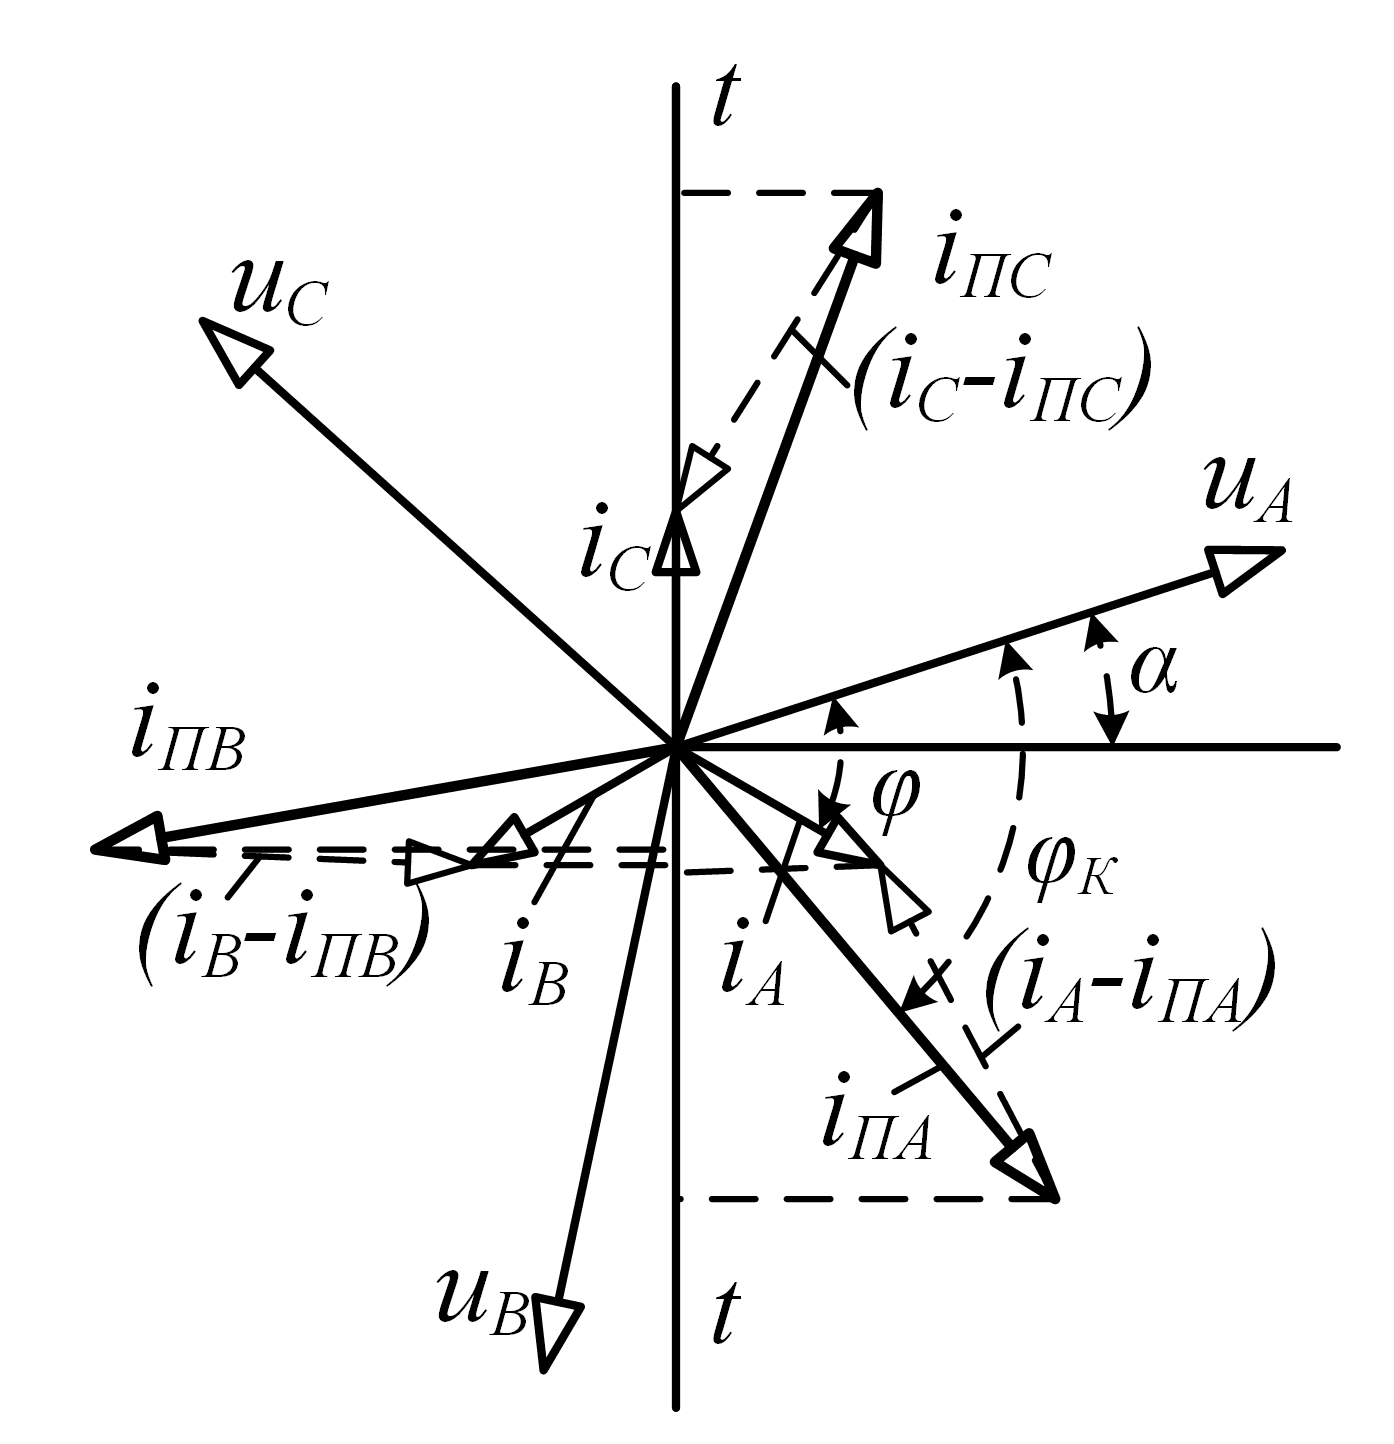
\includegraphics[width=0.40\linewidth]{pic/3-2}
	\caption{Векторная диаграмма для начального момента трехфазного короткого замыкания.}
	\label{ris:3-2 diagram}
\end{floatingfigure}

\begin{small}
	Напомним, что подкасательная в любой точке экспоненты\footnote{Обычно используют начальную часть экспоненты, где скорость изменения соответствующей величины больше и поэтому можно точнее провести касательную.} в принятом для оси времени масштабе дает значение постоянной времени, с которой происходит изменение экспоненты (рис. \colorbox{red}{3-3}). Имея в виду, что при $ t = T_{\text{а}} $ значение $ e^{-1} = 0,368 $, постоянную $ T_{\text{а}} $ обычно трактуют как время, в течение которого переменная величина снижается до 0,368 своего начального значения; при этом за начальную может быть принята любая точка кривой.
	
\end{small}

%TODO: Рисунок оказывается перед 3-2 ??!!
\begin{figure}
	\center{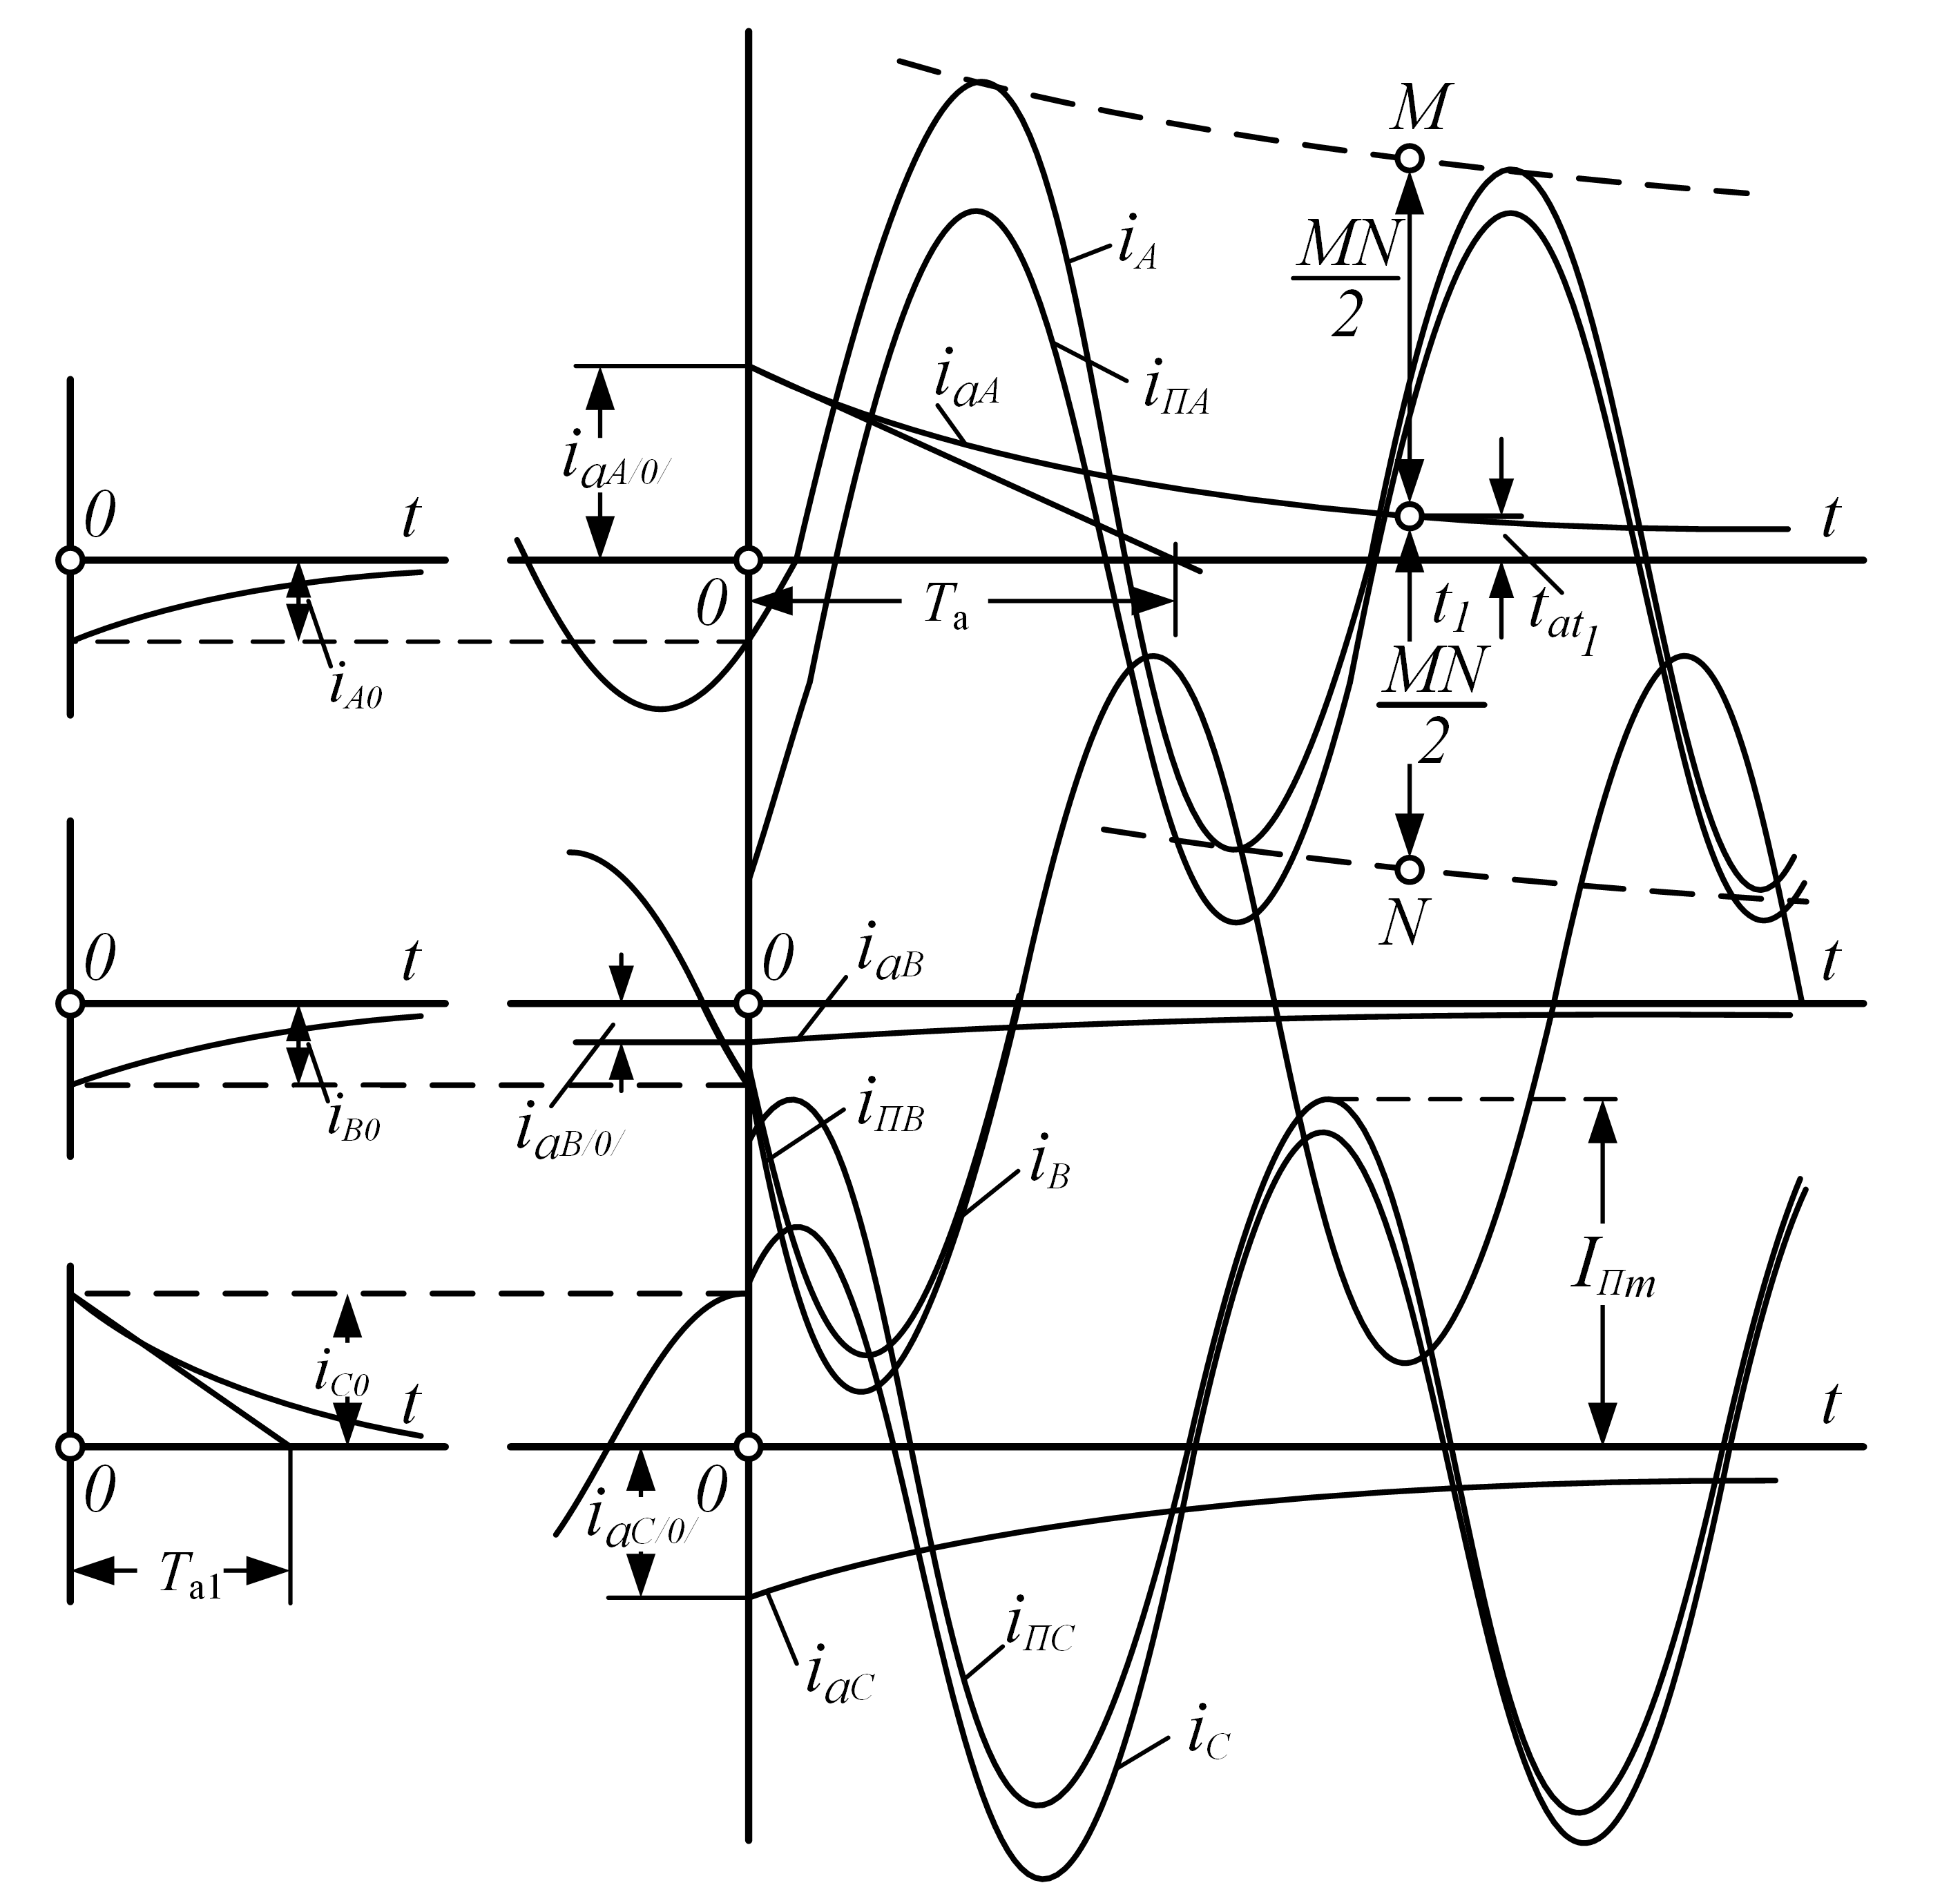
\includegraphics[width=0.85\linewidth]{pic/3-3}}
	\caption{Осциллограммы токов в фазах при внезапном трехфазном коротком замыкании в простейшей электрической цепи.}
	\label{ris:3-3}
\end{figure}

Перейдем теперь к участку цепи, который остался присоединенным к источнику. Здесь помимо свободного тока будет новый принужденный ток, величина которого, очевидно, больше предыдущего и сдвиг по фазе которого в общем случае иной. Допустим, что векторы $ I_{\text{П}A} $, $ I_{\text{П}B} $, $ I_{\text{П}C} $ (рис.~\ref{ris:3-2 diagram}) отвечают новому установившемуся режиму данного участка цепи.

Дифференциальное уравнение равновесия для любом фазы, например фазы \textit{А}, этого участка

\begin{equation*}
	u_A = i_A r_{\text{К}} + L \frac{di_A}{dt} + M \frac{di_B}{dt} + M \frac{di_C}{dt},
\end{equation*}

имея ввиду, что $ (i_B + i_C) = -i_A $, можно представить (опуская индекс фазы) как

\begin{equation}	
	u = i r_{\text{К}} + L_{\text{К}} \frac{di}{dt},
	\tag{\ref*{eq:3-1 diff_ur}а}
	\label{eq:3-1a u}
\end{equation}

где $ L_{\text{К}} = (L - M) $ --- результирующая индуктивность фазы, т.~е. индуктивность с учетом влияния двух других фаз.

Решение (\ref{eq:3-1a u}) имеет вид:

\begin{equation}	
	i = \frac{U_m}{z_{\text{К}}} sin(\omega t + \alpha - \varphi_{\text{К}}) + i_{\text{а} | 0 |} e^{-t / T_{\text{а}}}
	\tag{\ref*{eq:3-2 diff_solve}а}
	\label{eq:3-2a i}
\end{equation}

где $ z_{\text{К}} $ --- полное сопротивление присоединенного к источнику участка цепи или. короче, цепи короткого замыкания;

$ \varphi_{\text{К}} $ --- угол сдвига тока в этой цепи;
	
$ T_{\text{a}} $ --- постоянная времени цепи короткого замыкания, определяемая по (\ref{eq:3-3 T_a1}), где вместо $ L_1 $, $ x_1 $, $ r_1 $ следует ввести $ L_{\text{К}} $, $ x_{\text{К}} $, $ r_{\text{К}} $.

Первый член правой части (\ref{eq:3-2a i}) представляет периодическую слагающую тока, которая при рассматриваемых условиях является принужденным током с постоянной амплитудой $ I_{\text{П}m} = U_m / z_{\text{К}} $. Соответственно второй член представляет, как и раньше, затухающий по экспоненте свободный ток; его называют также апериодической слагающей тока. Начальное значение этой слагающей определяется из начальных условий, т.~е.

% В этом месте в книге опечатка, формула названа 3-3, нумерация дальше отличается
\begin{equation}
	i_0 = i_{\text{п}~/0/} + i_{\text{а}~/0/},
	\label{eq:3-4 i_0}
\end{equation}

откуда после подстановки соответствующих выражений имеем:

\begin{equation}
	i_{\text{а}|0|} = I_m sin(\alpha - \varphi) - I_{\text{П}m} sin(\alpha - \varphi_{\text{К}}).
	\label{eq:3-5 i_a0}
\end{equation}

Поскольку токи $ i_{\text{П}} $, $ i_0 $ являются проекциями векторов $ \overset{\;.}{I}_{\text{П}m} $ и $ \overset{\;.}{I}_m $ на линию времени, то ток $ 	i_{\text{а}|0|} $ также можно рассматривать как проекцию вектора $ (\overset{\;.}{I}_m - \overset{\;.}{I}_{\text{П}m} $ на ту же линию (рис.~\ref{ris:3-2 diagram}). В зависимости от фазы включения $ \alpha $ начальное значение тока $ 	i_{\text{а}|0|} $ может изменяться от возможной наибольшей величины, когда вектор $ (\overset{\;.}{I}_m - \overset{\;.}{I}_{\text{П}m} $ параллелен линии времени, до нуля, когда этот вектор нормален к ней. В трехфазной системе такие частные условия, разумеется, могут быть лишь в одной из фаз.

%TODO: Рисунок 3-4

На рис. \colorbox{red}{3-3} справа представлены кривые изменения токов в фазах рассматриваемого участка при трехфазном коротком замыкании. Как видно, чем больше апериодическая слагающая тока, тем больше смещение кривой полного тока относительно оси времени. Эту слагающую можно рассматривать как криволинейную ось симметрии кривой полного тока, из которой ее легко выделить. Для этого нужно сначала провести огибающие по максимальным положительным и отрицательным значениям заданной кривой тока (см. пунктирные линии у кривой тока фазы \textit{А} на \colorbox{red}{рис. 3-3}). Каждая точка кривой апериодической слагающей лежит посредине вертикального отрезка между этими огибающими.

Из (\colorbox{red}{3-4}) и рис. \colorbox{red}{3-2} следует, что наибольшее значение апериодической слагающей тока определяется не только фазой включения, но также предшествующим режимом цепи. Так, например, при отсутствии предшествующего тока в данной цепи величина 
при отсутствии величина $ i_{\text{а}/0/} $ может достигать амплитуды периодической слагающей, если в момент короткого замыкания эта слагающая проходит через свой положительный или отрицательный максимум (рис.\colorbox{red}{3-4}). Обычно этот случай рассматривается как расчетный\footnote{Хотя возможны частные случаи, когда начальное значение апериодической слагающей тока превышает амплитуду периодической слагающей.}.

Важно отметить, что фаза включения, при которой возникает наибольшее значение апериодической слагающей, еще не предопределяет того, что именно при ней будет максимум мгновенного значения полного тока. В самом деле, из (\ref{eq:3-2a i}) и (\ref{eq:3-5 i_a0}) при отсутствии предшествующего тока ($ I_m = 0 $) следует, что полный ток в цепи короткого замыкания является функцией двух независимых переменных: времени $ t $ и фазы включения $ \alpha $ и выражается уравнением










\bibliographystyle{unsrt} % сортировка литературы в порядке упоминания (не как в книге)
\bibliography{./tex/lit}
\addcontentsline{toc}{chapter}{\bibname}

\backmatter
% bibliography, glossary and index would go here.

\end{document}